\subsection{Models Trained on EHR Data}
The first iteration of the experiment consisted of training RF, SVM, and LUCCK models on EHR data to predict an increase in qSOFA score after a prediction gap. The results of the voting system on the test set are presented in Figure (TODO: Remove ehrOnly) for 6- and 12-hour gap. The vertical bars indicate the mean value after 100 iterations, and the error bars, one SD.

\subsection{Models Trained on Tensor-Reduced Signal Features}
RFs were trained on tensor-reduced ECG features, presented in Table \ref{fig:rf_ecgonly}, and these models are compared to those trained on tensor-reduced ECG features and arterial line features, presented in Table \ref{fig:rf_sigonly}. These figures display the mean F1 Score and AUROC over 100 iterations, with error bars indicating one SD. The $x$-axis indicates the rank selected for CP-ALS. Rank 1 is omitted as it consistently had inferior performance compared to other results. This may be the result of too much reduction, where information is lost in addition to noise.

Results of RF models trained on both the tensor-reduced signal features and EHR data are presented in Figure \ref{fig:rf_sigEHR}.

A comparison between RF models trained on tensor-reduced arterial line and ECG signal features and RF trained on EHR features for prediction gaps of 6 and 12 hours is included in Supplementary Materials Section 1.3. These results are those from Figures (TODO: Remove ehrOnly) and \ref{fig:rf_sigonly}, placed alongside each other to show the similarity in results.

% jonathan: I don't think the additional rank results contribute to the paper - I would only have no tensor reduction vs the best performing rank
\begin{figure}[htb]
    \centering
    \begin{subfigure}[htb]{0.49\textwidth}
        \includegraphics[width=\textwidth]{body/figures/ecg_6.svg}
    \end{subfigure}
    \hfill
    \begin{subfigure}[htb]{0.49\textwidth}
        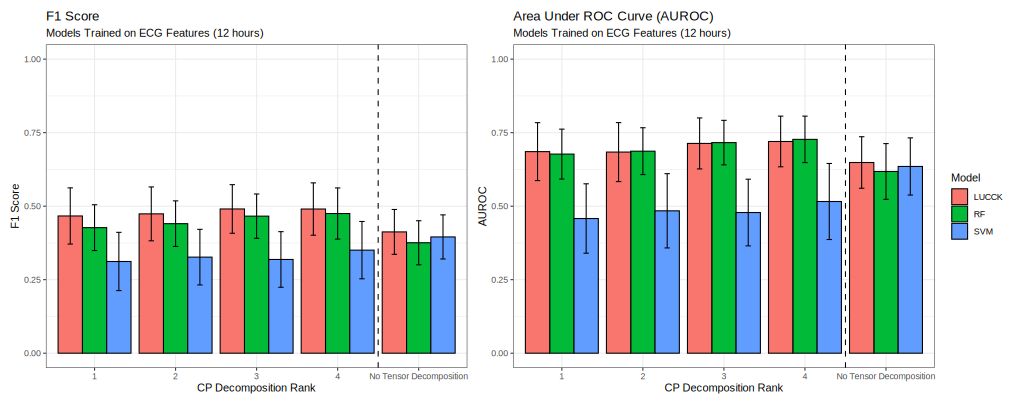
\includegraphics[width=\textwidth]{body/figures/ecg_12.svg}
    \end{subfigure}
    \caption{Models using ECG}
    \label{fig:rf_ecgonly}
\end{figure}  % ECG random forest

\begin{figure}[htb]
    \centering
    \begin{subfigure}[htb]{0.49\textwidth}
        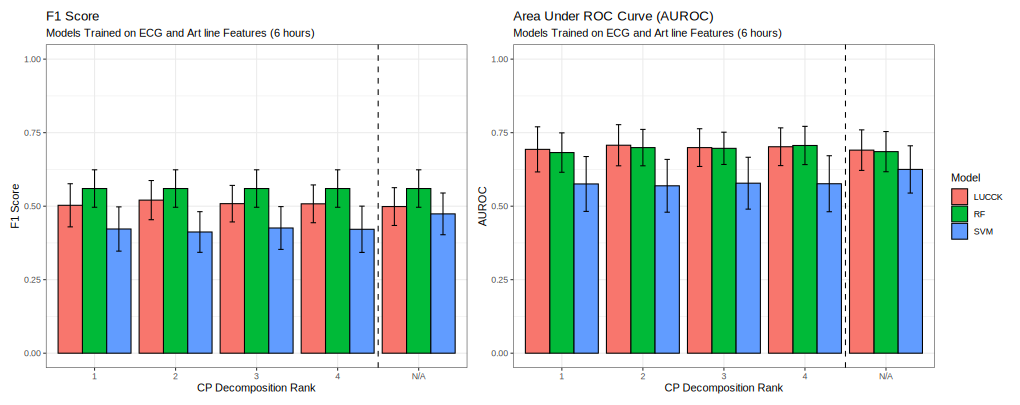
\includegraphics[width=\textwidth]{body/figures/both_6.svg}
    \end{subfigure}
    \hfill
    \begin{subfigure}[htb]{0.49\textwidth}
        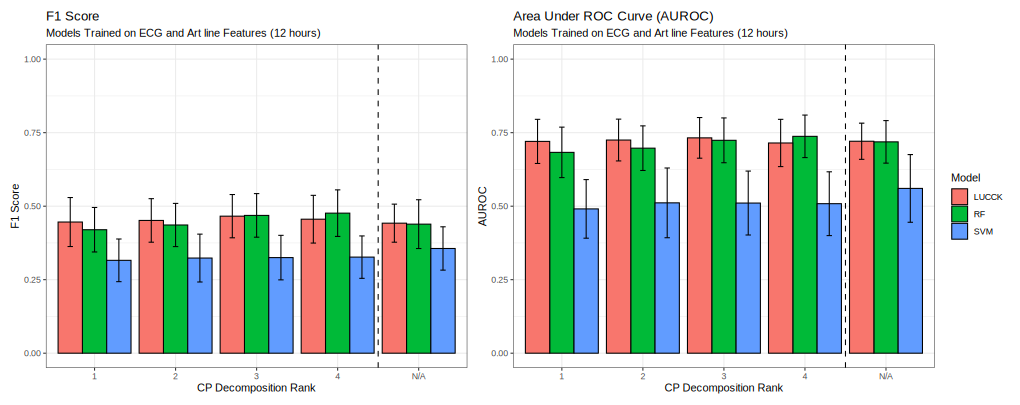
\includegraphics[width=\textwidth]{body/figures/both_12.svg}
    \end{subfigure}
    \caption{RF using Arterial Line and ECG}
    \label{fig:rf_sigonly}
\end{figure}  % ART + ECG random forest

\begin{figure}[htb]
    \centering
    \begin{subfigure}[htb]{0.49\textwidth}
        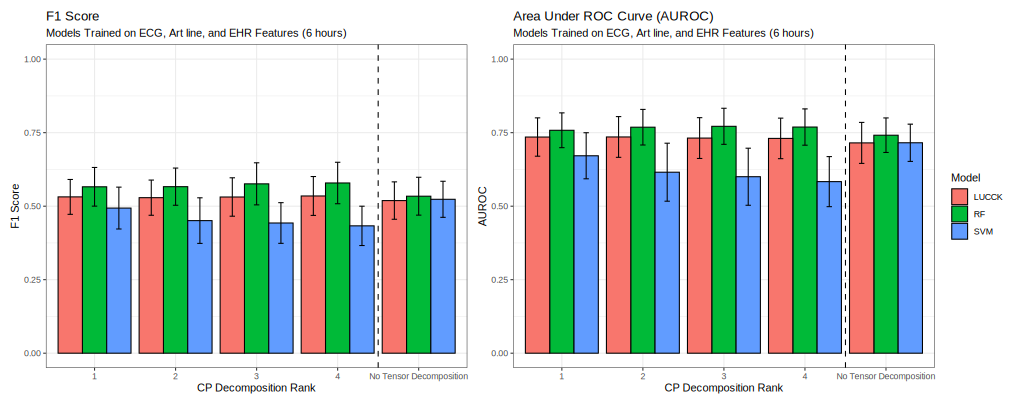
\includegraphics[width=\textwidth]{body/figures/all_6.svg}
    \end{subfigure}
    \hfill
    \begin{subfigure}[htb]{0.49\textwidth}
        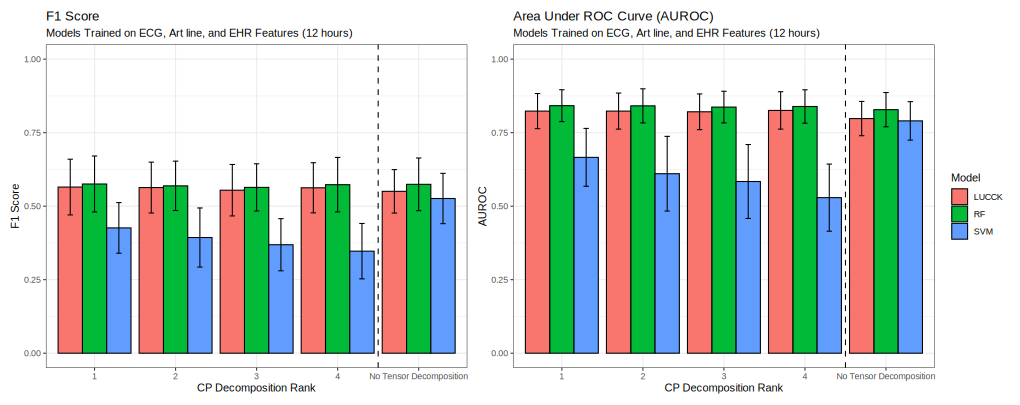
\includegraphics[width=\textwidth]{body/figures/all_12.svg}
    \end{subfigure}
    \caption{RF using Arterial Line, ECG, and EHR Data}
    \label{fig:rf_sigEHR}
\end{figure}  % ART + ECG + EHR random forest

\clearpage